\section{Introduction}
\index{Probabilistic Risk!Event-Based}
The probabilistic event-based risk calculator uses \glspl{stochasticeventset} and associated \glspl{groundmotionfield} to compute loss exceedance curves for each \gls{asset} contained in an \gls{exposure model}. This calculator thus requires \glspl{groundmotionfield} from a number of stochastic events as an input, which the engine can calculate using the oq-hazardlib.

For each \glspl{groundmotionfield}, the intensity measure level at a given site is combined with a \gls{vulnerability function}, from which a loss ratio is randomly sampled, for each \gls{asset} contained in the \gls{exposure model}. The loss ratios that are sampled for \glspl{asset} of a given \gls{taxonomy} classification at different locations are considered to be either independent or correlated. The losses for a given asset are calculated using all of the \glspl{groundmotionfield}, leading to list of events and associated loss ratios. This list is then sorted from the highest loss ratio to the lowest. The rate of exceedance of each loss ratio is calculated by dividing the number of exceedances of that loss ratio by the number of \glspl{stochasticeventset} multiplied by the length of each event set. By assuming a Poissionian distribution of the occurrence model, the probability of exceedance of each loss ratio is calculated. If a total loss curve for a portfolio of \glspl{asset} is required, a secondary module is used in order to sum the losses from all the \glspl{asset} in the exposure file, per event, before calculating the exceedance distribution of loss. This distribution of the total losses per event can also be extracted, and it is termed here as an \gls{eventLossTable}.

Similarly to what has been described for the Scenario Risk Calculator (see section \ref{chap:scenario_risk}), this module can compute \gls{insuredLosses} following the same approach (i.e. modifying the  loss based on the \gls{deductible} and \gls{limit} for each cost type).

This calculator is also capable of performing \gls{lossdisaggregation} in terms of magnitude/distance or latitude/longitude. In order to do so, the losses at each location are disaggregated based on the aforementioned parameters, and a loss percentage for each possible combination is calculated.

\section{Calculation Steps}

To compute the loss exceedance curves:

\begin{enumerate}
\item The oq-engine starts by using the set of \glspl{groundmotionfield} to extract the intensity measure levels for the location of each \gls{asset}. 
 
\item Then the oq-engine takes the \gls{vulnerability function} assigned to each \gls{asset} and checks if the coefficient of variation is zero. If so, the loss ratios are derived based on the mean loss ratio for each intensity measure level. Otherwise, if the uncertainty is defined, it is randomly sampled following the probabilistic distribution, mean loss ratio and associated coefficient of variation of the respective function, as described below:

\begin{equation}
\log{LR_n} = \mu + \epsilon\sigma
\end{equation}

Where $\mu$ and $\sigma$ stand for the mean and standard deviation of the logarithm of the loss ratios respectively and $\epsilon$ is a term that has a standard normal distribution with a zero mean and a standard deviation of one.  

The method used to sample epsilon can follow tree approaches depending on whether the correlation between the vulnerability of \glspl{asset} of a given \gls{taxonomy} is to be considered or not:

\begin{itemize}

\item Perfectly correlated: the term $\epsilon$ is randomly sampled once for the first \gls{asset} and this result is used to derive the loss ratio for all the \glspl{asset} of the same \gls{taxonomy}. 

\item Correlated: the term $\epsilon$ is randomly sampled for each \gls{asset} considering the specified correlation coefficient between \glspl{asset}. 

\item Uncorrelated: the term $\epsilon$ is always randomly sampled for each \gls{asset} and therefore the correlation between the vulnerability of the \glspl{asset} is ignored.
\end{itemize}

\item Each loss ratio is multiplied by the associated asset value, leading to the absolute loss values. If these losses are related with the structural, non-structural or contents cost, the \gls{insuredLosses} module can be used to modify the \gls{groundupLosses} according to the associated \gls{deductible} and \gls{limit} thresholds, as described in section \ref{chap:scenario_risk}.

\item In this method the losses to each \gls{asset} for each event are estimated and then sorted from highest to lowest. The rate of exceedance of each loss is calculated by dividing the number of exceedances of that loss by the number of \glspl{stochasticeventset} multiplied by the length of each event set. Hence, the top loss will have zero exceedances, the next loss ratio will have one exceedance, and so on.

The following formula is employed to compute the rate of exceedance:

\begin{equation}
\lambda(L_n) = \frac{NE_{L}}{TSES}
\end{equation}

Where  $\lambda$ stands for the rate of exceedance of the respective loss ratio, $NE_{L}$ stands for the number of exceedances of the given loss, and $TSES$ stands for the time span of all \glspl{stochasticeventset}, i.e. the number of \glspl{stochasticeventset} multiplied by the time span of each.

\item Assuming a Poissonion distribution of the occurrence model, the probability of exceedance of the set of losses in a given time span can be derived using the following formula:

\begin{equation}
PE(L_n) = 1-\exp{-\lambda_n\times t}
\end{equation}

Where $t$ stands for the time span used to produce the \gls{stochasticeventset}.

\end{enumerate}

To perform the loss disaggregation:

\begin{enumerate}

\item For the disaggregation of the losses it is necessary to provide the coordinates of the locations where this procedure should be employed. Then, for the selected locations, the oq-engine calculates the sum of the losses (considering all the assets existing at each of the selected sites) for each seismic event. In addition, the rupture distance (Joyner-Boore) and coordinates of the point within the vertical projection of the rupture plane closest to each site are estimated. An example of this type of information is presented in Figure \ref{fig:SetLosses}, for 20 stochastically produced seismic events.

\begin{figure}[ht]
\centering
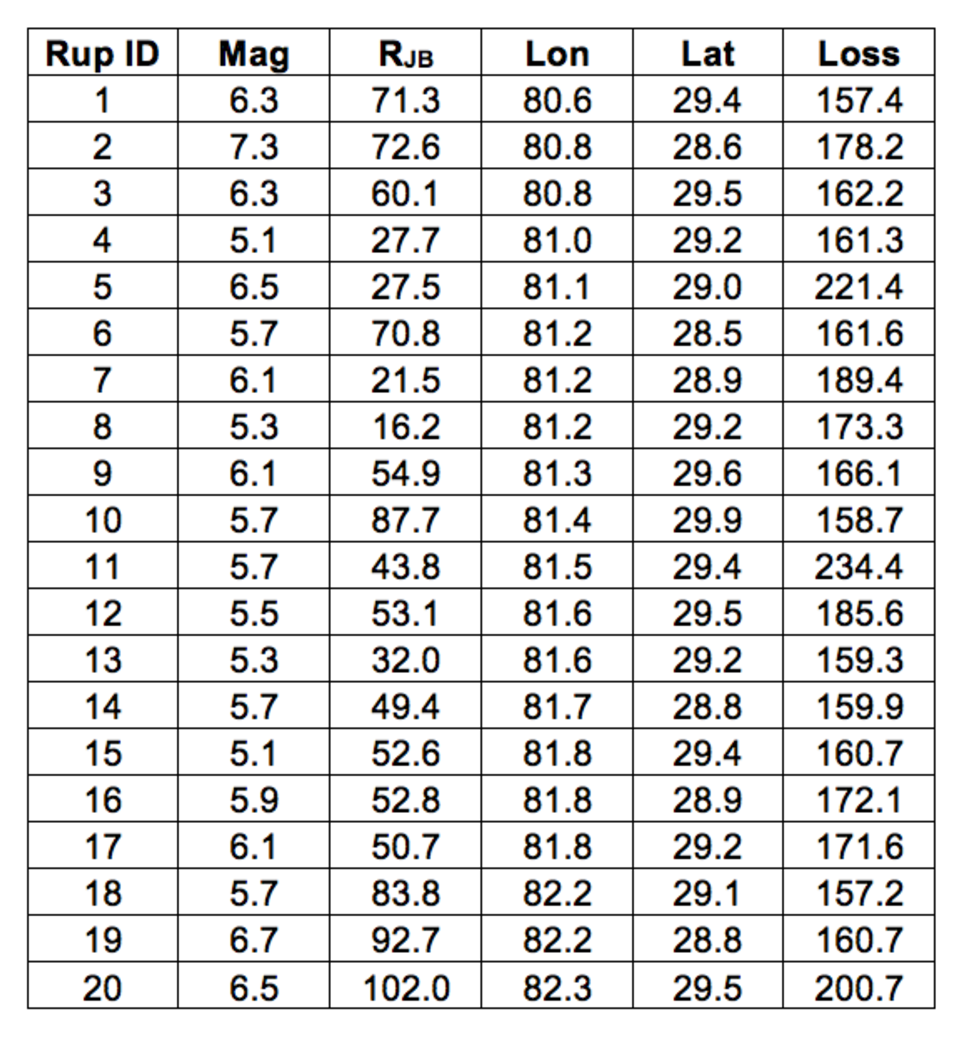
\includegraphics[width=9cm,height=10cm]{./figures/risk/SetLosses.eps} 
\caption{Economic losses from a single asset for a set of seismic events.}
\label{fig:SetLosses}
\end{figure} 

\item The oq-engine calculates the range (maximum and minimum values) of the list of magnitudes, distances, latitudes and longitudes across all the events, and using the increment defined for each parameter, a set of linearly spaced bins is calculated. Then, the losses from every seismic event are aggregated depending into which combination of magnitude/distance or latitude/longitude they fall. The previously presented losses have been disaggregated according to these two combinations as presented in Figure \ref{fig:Dis}:

\begin{figure}[ht]
\centering
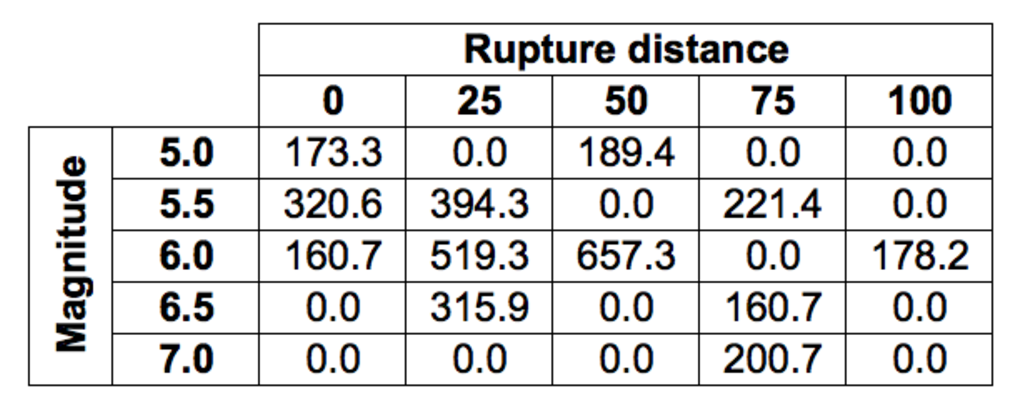
\includegraphics[width=8cm,height=3cm]{./figures/risk/DisaggregationDistMag.eps} 
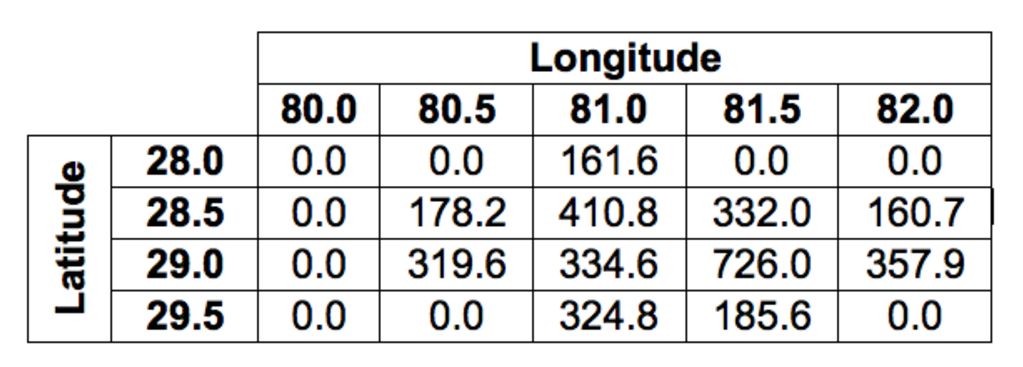
\includegraphics[width=8cm,height=2.8cm]{./figures/risk/DisaggregationCoor.eps} 
\caption{Disaggregation of the economic losses according to a set of magnitude/distance and latitude/longitude combinations.}
\label{fig:Dis}
\end{figure} 

\item The resulting losses for each pair of parameters (magnitude/distance and latitude/longitude) are divided by the total loss across all the events. This percentage of the overall loss for each combination is depicted in Figure \ref{fig:disaggregation} in the following section.
\end{enumerate}

\section{Calculator Output}
The output of this calculator comprises loss exceedance curves and loss maps. Loss exceedance curves are represented by a list of losses and respective probabilities of exceedance. Furthermore, each curve is associated with a pair of coordinates, an end branch label (that allows the curve to be connected to the set of specifications used in the calculations) and an asset ID (that permits tracking of the asset that each loss curve was computed for). Loss maps for a given probability of exceedance in a given time span can be produced, as well as maps of mean loss within a given time span. Figure \ref{fig:LossCurve01} and \ref{fig:LossCurve001} present a loss map for a probability of exceedance of 1\% and 10\% in 50 years for residential buildings located in Nepal, respectively. 

\begin{figure}[H]
\centering
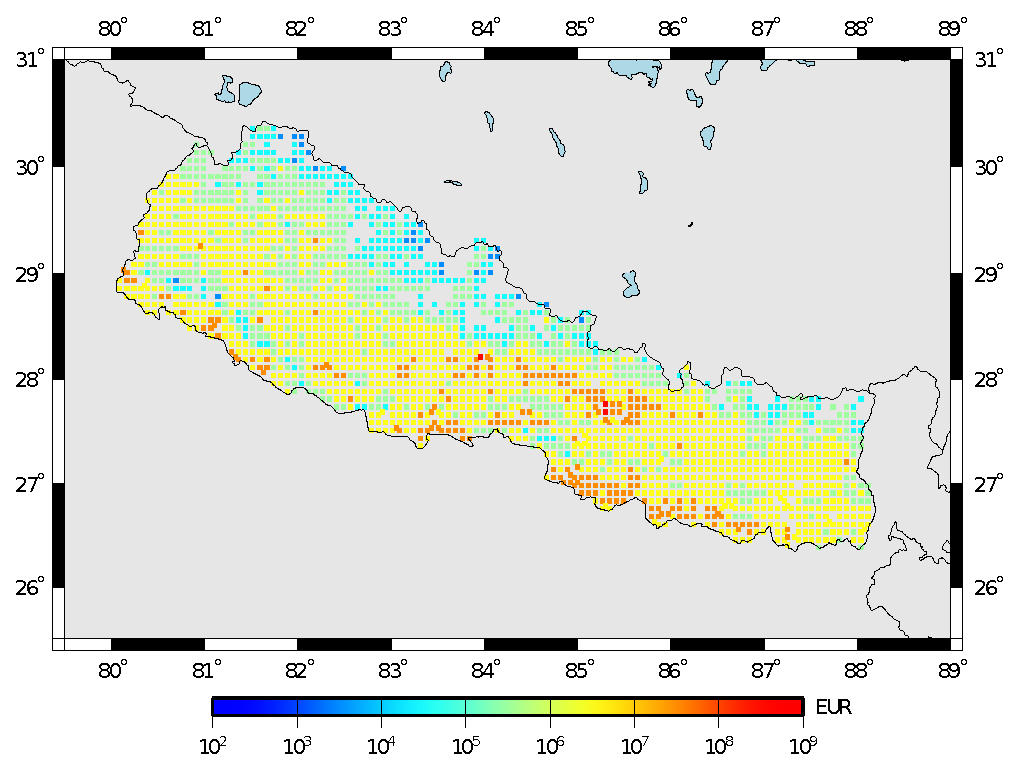
\includegraphics[width=12cm,height=8cm]{./figures/risk/LossMap01.eps} 
\caption{Loss map for a probability of exceedance of 10\% in 50 years.}
\label{fig:LossCurve001}
\end{figure} 

\begin{figure}[H]
\centering
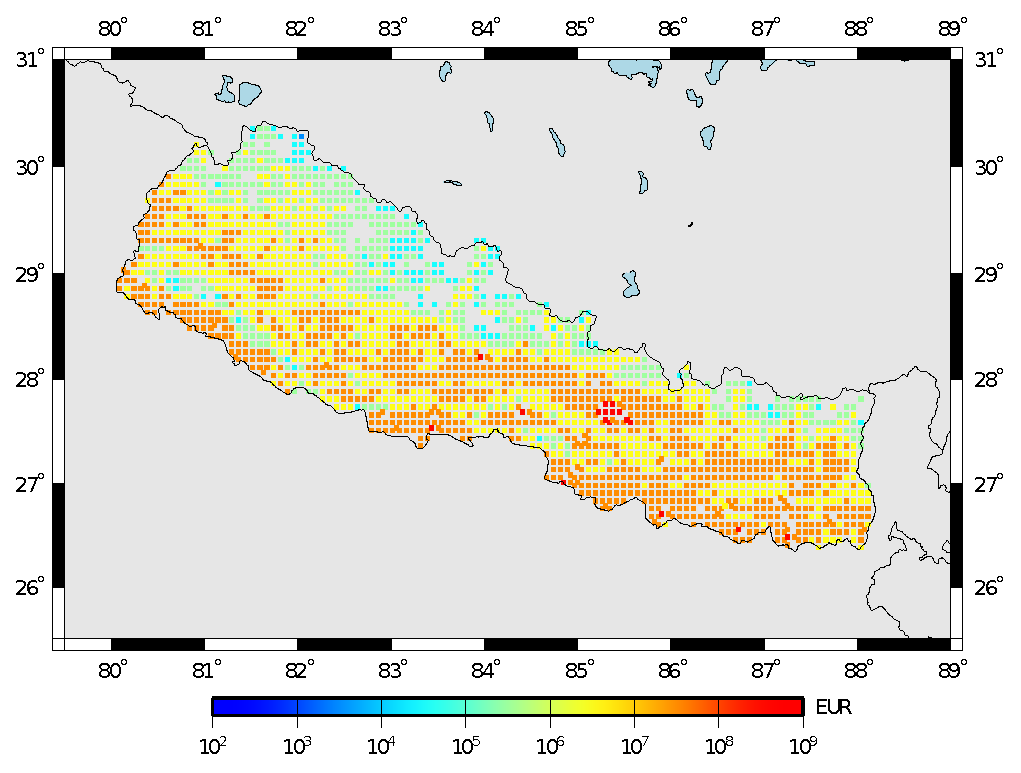
\includegraphics[width=12cm,height=8cm]{./figures/risk/LossMap001.eps} 
\caption{Loss map for a probability of exceedance of 1\% in 50 years.}
\label{fig:LossCurve01}
\end{figure} 

For this calculator, total loss exceedance curves can be produced which combine the losses to all \glspl{asset} per event. It is noted that loss exceedance curves which present the probability of exceedance of the aggregate annual losses, or maximum annual losses, are not yet supported in the oq-risklib. In Figure \ref{fig:ProbLosses}, a total loss exceedance curve for the residential building portfolio in Nepal is presented. 
 
\begin{figure}[H!]
\centering
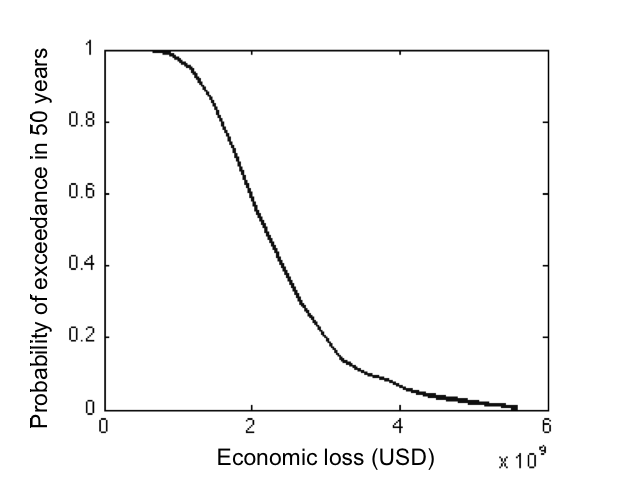
\includegraphics[width=8cm,height=6cm]{./figures/risk/LossCurveIstanbul.eps}
\caption{Total loss exceedance curve for RC buildings.}
\label{fig:ProbLosses}
\end{figure} 

For what concerns the \glspl{eventLossTable}, the oq-engine can extract the total loss across all the assets for each seismic event. The results is a table with the rupture id, magnitude and total loss, as illustrated in Figure \ref{fig:eventLossTable}.

\begin{figure}[H!]
\centering
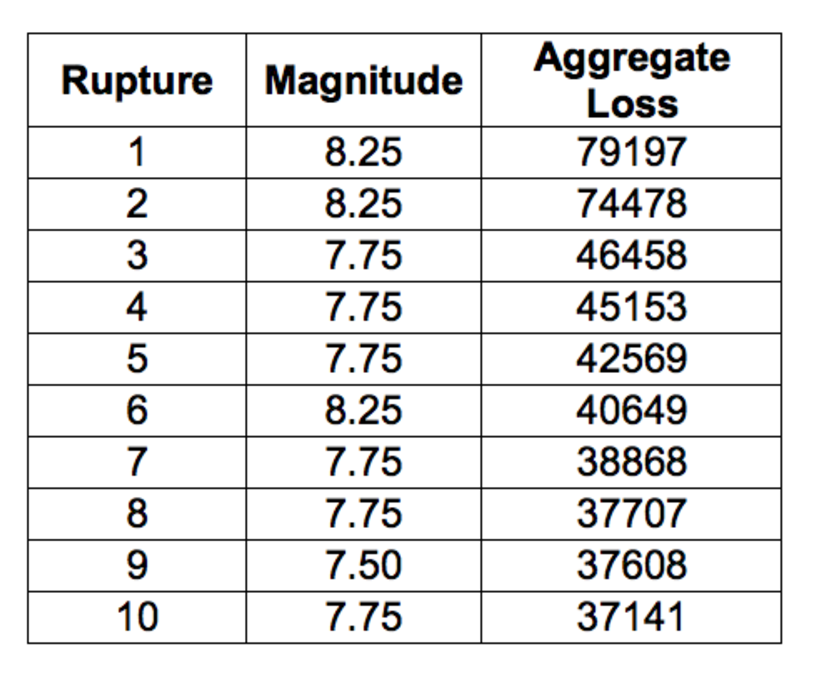
\includegraphics[width=6cm,height=5cm]{./figures/risk/EventLossTable.eps}
\caption{Example of an \gls{eventLossTable}.}
\label{fig:eventLossTable}
\end{figure} 

The output of the \gls{lossdisaggregation} is composed by the loss fraction associated to each combination of parameters (magnitude/distance or latitude/longitude), as presented in Figure \ref{fig:disaggregation} .

\begin{figure}[H!]
\centering
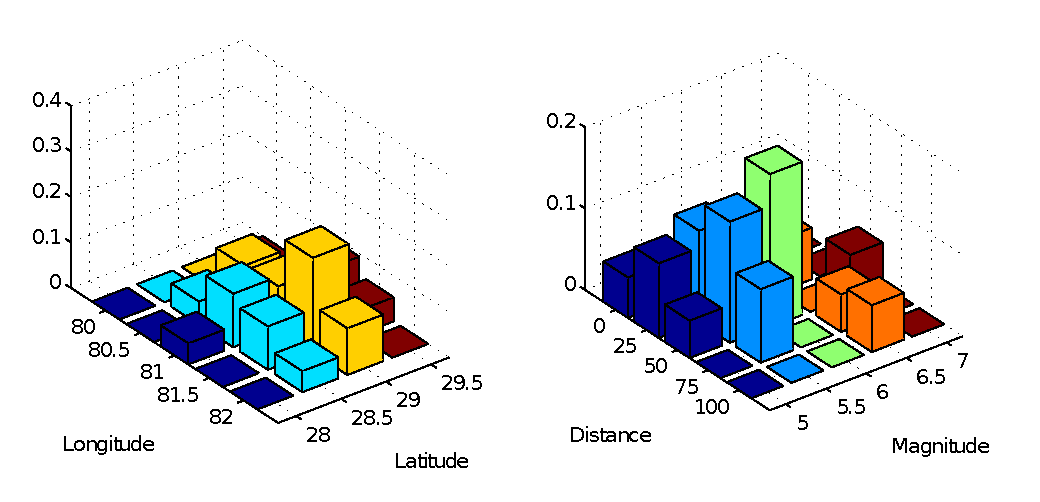
\includegraphics[width=14cm,height=6.5cm]{./figures/risk/Disaggregation.eps}
\caption{Example of a loss disaggregation according to a set of magnitude/distance and latitude/longitude combinations.}
\label{fig:disaggregation}
\end{figure} 
